\documentclass[12pt]{article}
\usepackage{graphicx}	% Used to for importing images
\usepackage{indentfirst}% Indents 1st paragraph (by default its off)
\usepackage{longtable} 	% Tables than can span over multiple pages
\usepackage{placeins}	% Used to keep images in place(via \FloatBarriers)
\usepackage{caption}	% Include captionof command for minipages

% Define Global Variables
\setlength{\parindent}{20pt}
\graphicspath{ {./Images} }

\begin{document}

\begin{titlepage}

% Defines a new command to draw horizontal lines
\newcommand{\Line}{\rule{\linewidth}{0.5mm}} 

% Center everything on the page
\center
 
% textsc - capitalizes every letter
\textsc{\LARGE University of Gothenburg}
% Define gap after text line
\\[3.5cm] 

% Course code and name
\textsc{\Large DIT168}\\[0.3cm]
\textsc{\large Project: Industrial IT and Embedded Systems}\\[0.5cm]
% Use the defined command to draw lines
\Line \\[0.4cm]
{\huge \bfseries User Manual}\\[0.4cm]
\Line \\[2cm]
 

\includegraphics[scale = 0.25]{Images/tab_logo.png}\\[2cm]	

{\large Group 01}\\
{\large May 20th, 2018}

% Fills the remaining page with whitespace
\vfill
\end{titlepage}

\tableofcontents
\pagebreak

%%%%%%%%%%%%%%%%%%%%%%%%%%%%%%%%%%%%%%%%%%%%%%%
%%% New Section
%%%%%%%%%%%%%%%%%%%%%%%%%%%%%%%%%%%%%%%%%%%%%%%
\section{Web Interface}
The developed interface, pictured in Figure \ref{fig:interface} can be divided to 3 sections; the remote control section, the sensor data visualization section and the message visualization section. \par
% Adding image
\FloatBarrier % -> Wrap image with this, to make sure text does not go infront of image if theres room
\begin{figure}[ht!]
\centering
% Make image as wide as the line
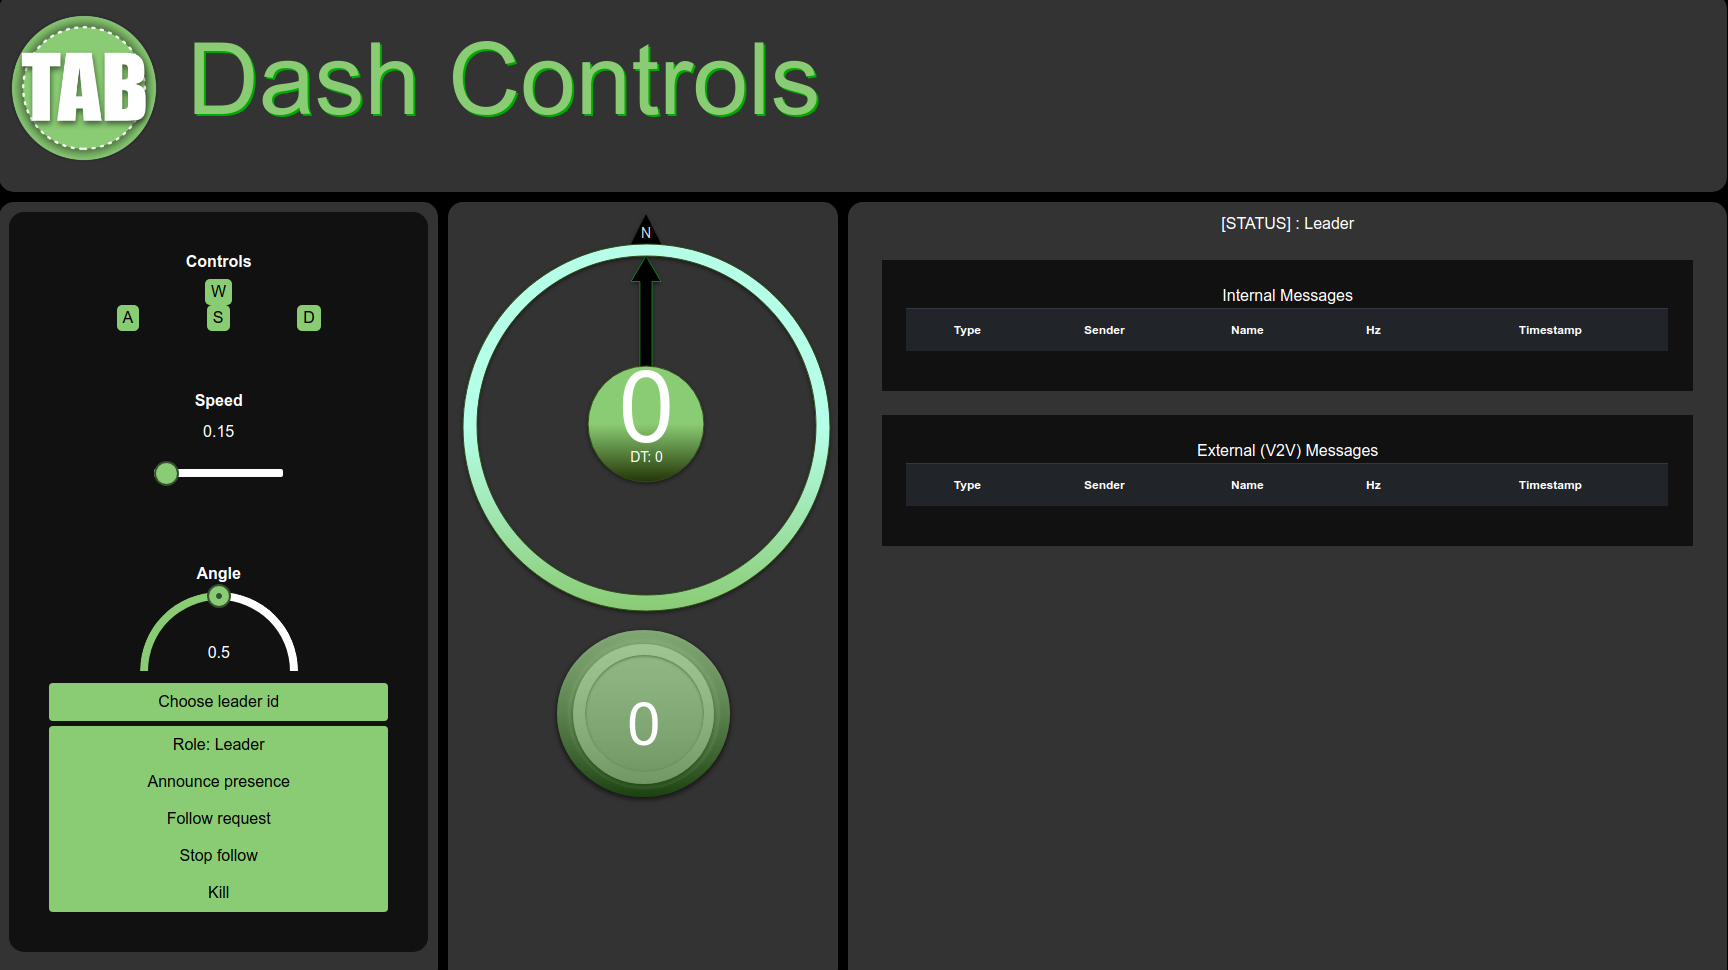
\includegraphics[width=\linewidth]{Images/whole_view.png}
\caption{Web Interface}
\label{fig:interface}
\end{figure}
\FloatBarrier % -> Wrap image with this, to make sure text does not go infront of image if theres room

The purpose of the interface, was to provided a nice and clean way of controlling the miniature vehicle. The development group though that the best way to achieve this is by using a single web page to provide both vehicle controls and data visualization.

%%%%%%%%%%%%%%%%%%%%%%%%%%%%%%%%%%%%%%%%%%%%%%%
%%% New Section
%%%%%%%%%%%%%%%%%%%%%%%%%%%%%%%%%%%%%%%%%%%%%%%
\section{Control Section}
\noindent
\begin{minipage}[t]{0.49\textwidth}
    \vspace{0pt} 
	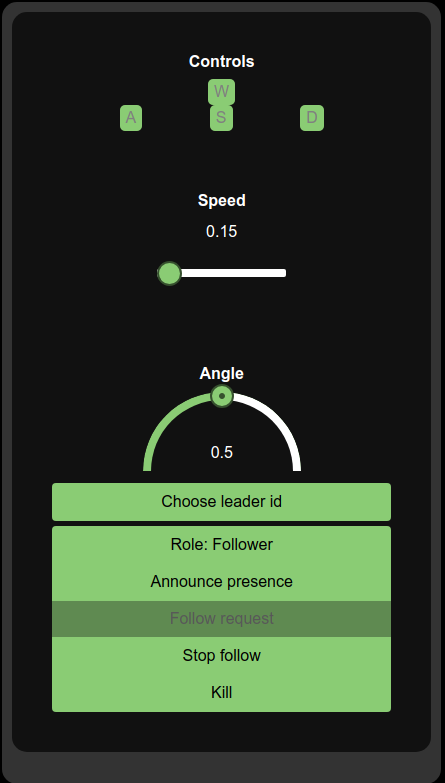
\includegraphics[width=\linewidth]{Images/control_section.png}
	\captionof{figure}{Control Section}
	\label{fig:control section}
\end{minipage}% No space between minipages to have them next to each other
\hspace{0.02\textwidth} % Adds gap between minipages
\begin{minipage}[t]{0.49\textwidth}
    \vspace{0pt}
    \setlength{\parindent}{20pt}
	The Control Section can be further divided into 2 separate sections or views. \par 
    The bottom section, discussed in section \ref{subsec:message controls} is used to control what kind of messages are sent from the miniature car. \par
    The top section, discussed in \ref{subsec:steering controls}, is used to provide steering controls to the user. \par
    This section of the manual is aimed to inform the user on how they can steer and control the car.
\end{minipage}% Make image as wide as the line

%%%%%%%%%%%%%%%%%%%%%%%%%%%%%%%%%%%%%%%%%%%%%%%
%%% New Section
%%%%%%%%%%%%%%%%%%%%%%%%%%%%%%%%%%%%%%%%%%%%%%%
\subsection{Message Controls} \label{subsec:message controls}
\noindent
\begin{minipage}[t]{0.49\textwidth}
    \vspace{0pt} 
	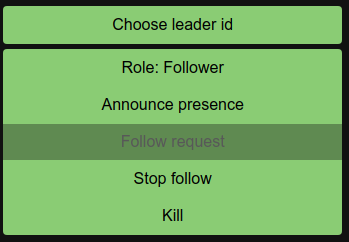
\includegraphics[width=\linewidth]{Images/message_control_small.png}
	\captionof{figure}[]{Message Controls}
	\label{fig:message controls small}
\end{minipage}% No space between minipages to have them next to each other
\hspace{0.02\textwidth} % Adds gap between minipages, h = horizontal
\begin{minipage}[t]{0.49\textwidth}
    \vspace{0pt}
   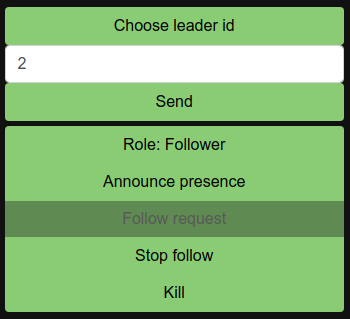
\includegraphics[width=\linewidth]{Images/message_control_full.png}
	\captionof{figure}{Message Controls}
	\label{fig:message controls full}  
\end{minipage}% Make image as wide as the line
\vspace{0.5cm} % Adds gap after minipage, v =vertical

The small panel, pictured in Figures \ref{fig:message controls small} \& \ref{fig:message controls full}, is used to provide the user, or the Driver of the miniature car, with controls over the V2V-Protocol. \par

The first button, "Choose leader id" is a drop-down button that allows the Driver to select which other miniature vehicle to attempt to connect to. The above figures are used to depict the difference between the button's selection states. Once the button is a selected the user will see a message field to enter the other cars' IDs and a button to send the new leader ID to the car. For this feature to work the other cars must have had announced their presence. This is due to the miniature cars storing the vehicle IPs within a map, the ID being the key and IP the value. Without the AnnouncePresence being sent the UDP Senders, Receivers could not be established. Hence no V2V following.\par

The second button, in Figure \ref{fig:message controls small} is used to swap between the miniature car's roles i.e. leader and follower. The current role is dispayed on the button itself and above the message visualization, seen in Figure \ref{fig:message section}. This button is significant, because the miniature car will not process some messages if it isn't in the correct role. For example, if the car is currently in Follower Mode the car will not execute LeaderStatus request if or when they are received.\par

The "Stop follow" and "Kill" button serve similar purposes. The Stop follow button, makes the miniature car send a StopFollow message disconnecting from the other car. After this a new connection can be established between the cars. The "Kill" button takes it a step further and turns of the V2V-Protocol after sending StopFollow message.\par

The "Announce presence" and "Follow request" buttons are not as significant. At previous iterations these buttons were used to control the sending of AnnouncePresence and FollowRequest messages respectively. However, currently the sending of these messages has been automated. The buttons have been left for testing and verification purposes. \par

%%%%%%%%%%%%%%%%%%%%%%%%%%%%%%%%%%%%%%%%%%%%%%%
%%% New Section
%%%%%%%%%%%%%%%%%%%%%%%%%%%%%%%%%%%%%%%%%%%%%%%
\subsection{Steering Controls} \label{subsec:steering controls}
\noindent
\begin{minipage}[t]{0.49\textwidth}
    \vspace{0pt} 
    \setlength{\parindent}{20pt}
	The figure right, focuses on the top section of Figure \ref{fig:control section}. Moreover, it depicts the Remote Controller created for the project. \par
    The Web Control provides the Driver control over 3 aspects; moving the car, changing car speed and altering turning angle. \par
    The Driver can move the car by pressing one of the "WASD" keys, pictured at the top of Figure \ref{fig:steering controls}. The choice for using "WASD" was motivated by its widespread use in gaming. Thus, it was believed that by incorporating these keys the development team could improve the intuitiveness of the remote controller. \par % Continues outside the minipage
\end{minipage}% No space between minipages to have them next to each other
\hspace{0.02\textwidth} % Adds gap between minipages, h = horizontal
\begin{minipage}[t]{0.49\textwidth}
    \vspace{0pt}
   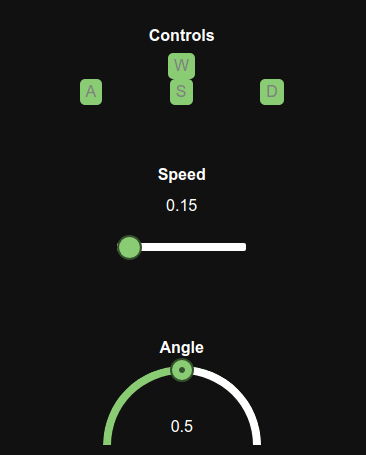
\includegraphics[width=\linewidth]{Images/steering_control.png}
	\captionof{figure}{Steering Controls}
	\label{fig:steering controls}  
\end{minipage}% Make image as wide as the line
\vspace{0.5cm} % Adds gap after minipage, v =vertical

To change the speed of the miniature car, the Driver can use the provided slider, with the current speed is displayed above the slider. The minimum speed is set to 0.15, due to it being the minimum required speed to physically move the car. The recommended speed range is between 0.15 and 0.20, as any higher could cause damage to the car's axis and cause the wheels to spin off. A second, curved slider is used to change the car's turning angle. The default is set to 0.5. These values correspond to percents.

%%%%%%%%%%%%%%%%%%%%%%%%%%%%%%%%%%%%%%%%%%%%%%%
%%% New Section
%%%%%%%%%%%%%%%%%%%%%%%%%%%%%%%%%%%%%%%%%%%%%%%
\section{Data Visualization}
The Web Interface is also responsible for data visualization, which can be split up in two parts; Sensors and Messages.

%%%%%%%%%%%%%%%%%%%%%%%%%%%%%%%%%%%%%%%%%%%%%%%
%%% New Section
%%%%%%%%%%%%%%%%%%%%%%%%%%%%%%%%%%%%%%%%%%%%%%%
\subsection{Sensors}
\noindent
\begin{minipage}[t]{0.4\textwidth}
    \vspace{0pt} 
	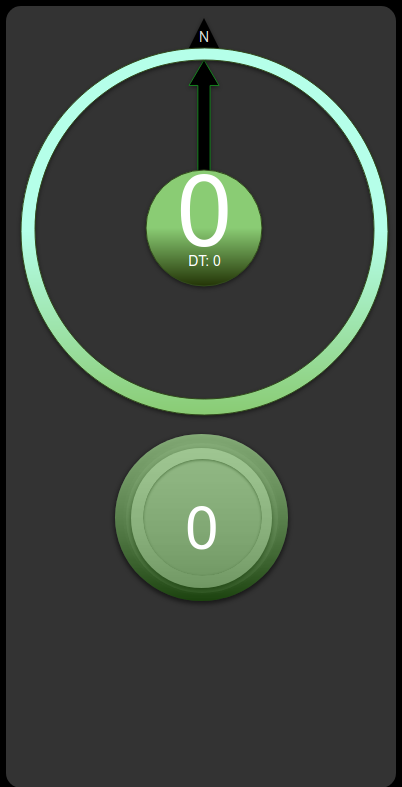
\includegraphics[width=\linewidth]{Images/sensors_section.png}
	\captionof{figure}{Sensor Section}
	\label{fig:sensor section}
\end{minipage}% No space between minipages to have them next to each other
\hspace{0.02\textwidth} % Adds gap between minipages
\begin{minipage}[t]{0.58\textwidth}
    \vspace{0pt}
    \setlength{\parindent}{20pt}
	The sensor section, pictured left, can be found in the middle of the interface as seen in Figure \ref{fig:interface}. This section is responsible for visualizing data from the IMU and the front Ultrasonic sensor.\par
    The larger circle, at the top of Figure \ref{fig:sensor section}, visualizes IMU readings. Specifically, 3 things. The first is the heading. These values are expressed as a compass with the black arrow pointing to the current car's heading. At the top of the circle a triangle with "N" meaning North. However, corresponds to the initial heading and is NOT affiliated with magnetic poles.\par
    A second smaller circle can be seen within the compass. The larger number is used to depict the current speed of the car, whereas the smaller number under it expresses the distance travelled by the car, hence the "DT:" in front the smaller value. \par
    The circle outside the compass is used to visualize Ultrasonic values. It changes colours from green to red. Red indicating that there is an object close to the car. The current distance to object is expressed as the number within the circle.
\end{minipage}% Make image as wide as the line

\subsection{Messages}
The messages being sent to and from the car are visualizesdin the right section on the interface. As mentioned in section \ref{subsec:message controls}, the current role of the car is depicted above the message visualization. 
% Adding image
\FloatBarrier % -> Wrap image with this, to make sure text does not go infront of image if theres room
\begin{figure}[ht]
\centering
% Make image as wide as the line
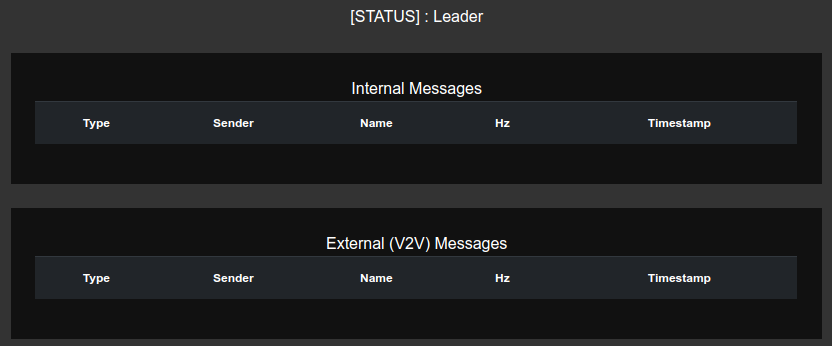
\includegraphics[width=\linewidth]{Images/message_section.png}
\caption{Message Visualization}
\label{fig:message section}
\end{figure}
\FloatBarrier % -> Wrap image with this, to make sure text does not go infront of image if theres room

%%%%%%%%%%%%%%%%%%%%%%%%%%%%%%%%%%%%%%%%%%%%%%%
%%% New Section
%%%%%%%%%%%%%%%%%%%%%%%%%%%%%%%%%%%%%%%%%%%%%%%
The message visualization is divided into two sections. The first being "Internal Messages". Under this table messages from all the developed microservices, except the V2V, can be seen. In other words steering messages and sensor messages. The second table, "External (V2V) Messages", visualizes all the messages sent by V2V-Protocol. \par

Once a message is received it creates a graph, pictured in Figure \ref{fig:message graph} . The graph is used to better visualize the change in the value being sent, in this case the role, over time. Additionally, the message ID, name, sender as well as its frequency and timestamp.
 % Adding image
\FloatBarrier % -> Wrap image with this, to make sure text does not go infront of image if theres room
\begin{figure}[h]
\centering
% Make image as wide as the line
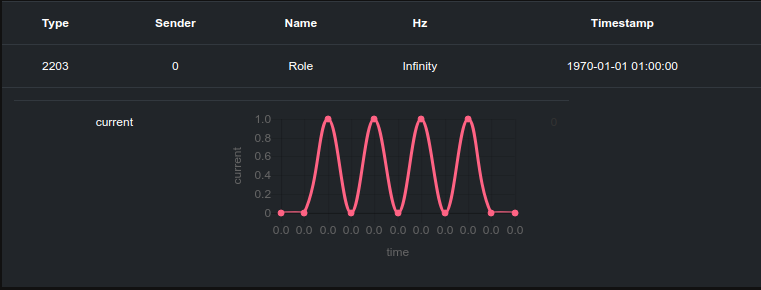
\includegraphics[width=\linewidth]{Images/message_role.png}
\caption{Message Graph}
\label{fig:message graph}
\end{figure}
\FloatBarrier % -> Wrap image with this, to make sure text does not go infront of image if theres room
\end{document}
